\documentclass[12pt]{article}			% For LaTeX 2e
						% other documentclass options:
						% draft, fleqn, openbib, 12pt

\usepackage{graphicx}	 			% insert PostScript figures
\usepackage{caption}
\usepackage{subcaption}
\usepackage{wrapfig}
\usepackage{amsmath}
%% \usepackage{setspace}   % controllabel line spacing
%% If an increased spacing different from one-and-a-half or double spacing is
%% required then the spacing environment can be used.  The spacing environment 
%% takes one argument which is the baselinestretch to use,
%%         e.g., \begin{spacing}{2.5}  ...  \end{spacing}


% the following produces 1 inch margins all around with no header or footer
\topmargin	=10.mm		% beyond 25.mm
\oddsidemargin	=0.mm		% beyond 25.mm
\evensidemargin	=0.mm		% beyond 25.mm
\headheight	=0.mm
\headsep	=0.mm
\textheight	=220.mm
\textwidth	=165.mm
					% SOME USEFUL OPTIONS:
% \pagestyle{empty}			% no page numbers
 \parindent  15.mm			% indent paragraph by this much
 \parskip     2.mm			% space between paragraphs
% \mathindent 20.mm			% indent math equations by this much

\newcommand{\MyTabs}{ \hspace*{25.mm} \= \hspace*{25.mm} \= \hspace*{25.mm} \= \hspace*{25.mm} \= \hspace*{25.mm} \= \hspace*{25.mm} \kill }

\graphicspath{{../Figures/}{../data/:}}  % post-script figures here or in /.

					% Helps LaTeX put figures where YOU want
 \renewcommand{\topfraction}{0.9}	% 90% of page top can be a float
 \renewcommand{\bottomfraction}{0.9}	% 90% of page bottom can be a float
 \renewcommand{\textfraction}{0.1}	% only 10% of page must to be text

\linespread{1.2}
\alph{footnote}				% make title footnotes alpha-numeric

\begin{document}			% REQUIRED

\noindent{\Large \bf 3 Integration and noise dampening using C-SVM}
\begin{figure}[h]
	\centering
	\includegraphics[scale=0.40]{img/wosvm.png}
	\caption{ \small Using conventional techniques, the noise present in the data forces constant log-outs on a false reject}
	\label{fig:sb2}
\end{figure}

\begin{figure}
	\centering
	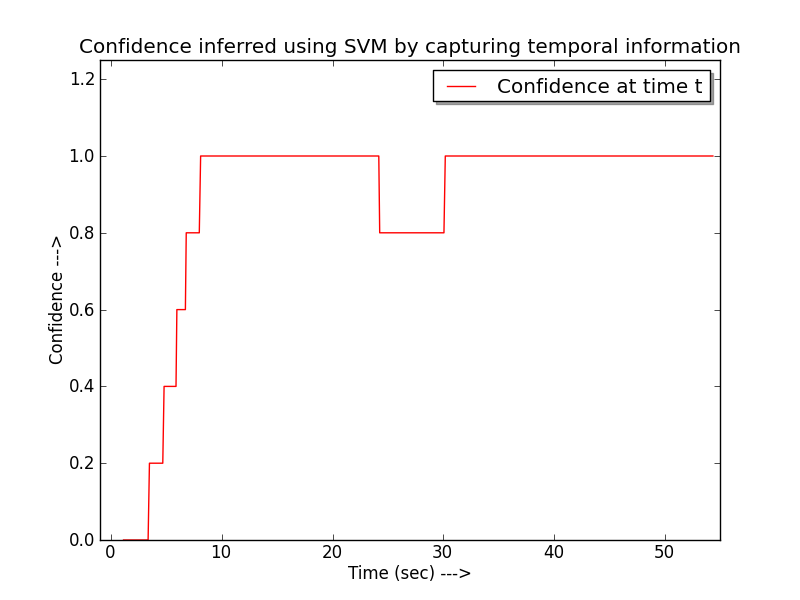
\includegraphics[scale=0.5]{img/svm.png}
	\caption{ \small By integrating an intelligent algorithm, in this case, a Support Vector Machine, we were able to drastically dampen noise by using temporal information to predict $P(X_{T}|X_{T-t})$ for every time period}
	\label{fig:sb2}
\end{figure}
\end{document}
